\section{最优解的存在}
\label{sec:opt-prob-existence}

上一节的$e^x$表明，最优值有限并不保证有点取得它。在讨论怎样求解之前，应当先确认所求的对象存在；否则一个算法“收敛”到的东西可能根本不是解。本节不构造任何算法，只问：一列越来越好的可行点，能否留下一个可行的极限，并把“好”传给这个极限。

\subsection{紧集与下半连续目标}
\label{sec:opt-prob-compact-lsc}

\paragraph{从最小化序列出发}
设$f^\star$有限。按下确界的定义，对每个$k$都有可行点$\bm x^{(k)}$满足$f(\bm x^{(k)})\leq f^\star+1/k$；若$f^\star=-\infty$，则改取$f(\bm x^{(k)})\leq-k$。这样的序列称为\term{最小化序列}（minimizing sequence），它的目标值趋于$f^\star$。这里的上标$(k)$只是序列编号，不表示任何算法的迭代。要从它得到最优解，需要依次完成三个环节：

\begin{enumerate}
  \item 序列有收敛的子列，即候选不会散开或逃向无穷远；
  \item 子列的极限仍然可行；
  \item 目标值的比较能传到极限，即极限处的目标值不高于序列目标值的极限。
\end{enumerate}

前两个环节由可行域负责，第三个环节由目标函数负责。在$\mathbb R^d$中，有界闭集的每个序列都有收敛子列，且极限仍在集合内，即有界闭集是紧集；这正好完成前两个环节（可参考\BookChapterRef{chap:metric-spaces}{卷二“度量空间”章}中紧致性的序列刻画与欧氏空间的闭有界判据）。第三个环节若用连续性完成，就得到熟悉的结论：有界闭集上的连续函数取得最小值，卷一已经在多元函数中建立（可参考\BookChapterRef{chap:multivariate-calculus}{卷一“多元函数微分”章}）。

\paragraph{只需要单向的比较}
仔细看第三个环节：我们只需要极限处的值“不比序列高”，不需要它“等于序列的极限”。函数可以在极限点向下跳，那只会让极限点更好；不能允许的是向上跳。这个单向条件就是下半连续性。

\begin{definition}[下半连续]
\label{def:opt-prob-lsc}
设$C\subseteq\mathbb R^d$，$f:C\to\mathbb R\cup\{+\infty\}$。若对$C$中每个收敛到$\bm x\in C$的序列$\bm x^{(k)}$，都有
\[
  f(\bm x)\leq\liminf_{k\to\infty}f(\bm x^{(k)}),
\]
就称$f$在$C$上\term{下半连续}（lower semicontinuous）。
\end{definition}

连续函数满足这个条件且取等号。下半连续还可以用“水平以下的部分”来刻画，这一刻画在下一小节是关键工具。对实数$a$，称$\{\bm x\in C:f(\bm x)\leq a\}$为$f$的\term{下水平集}（sublevel set），即地形图上高度不超过$a$的区域。

\begin{lemma}[下半连续与闭下水平集]
\label{lem:opt-prob-lsc-sublevel}
设$C\subseteq\mathbb R^d$闭，$f:C\to\mathbb R\cup\{+\infty\}$。$f$在$C$上下半连续，当且仅当对每个$a\in\mathbb R$，下水平集$\{\bm x\in C:f(\bm x)\leq a\}$是$\mathbb R^d$中的闭集。
\end{lemma}

\begin{proof}
设$f$下半连续，$\bm x^{(k)}$属于水平$a$的下水平集且收敛到$\bm x$。$C$闭，所以$\bm x\in C$；由下半连续，$f(\bm x)\leq\liminf_kf(\bm x^{(k)})\leq a$，极限仍在下水平集中，故下水平集闭。

反过来，设各下水平集都闭，但$f$在某点$\bm x\in C$不满足下半连续：存在$C$中的序列$\bm x^{(k)}\to\bm x$，使$\liminf_kf(\bm x^{(k)})<f(\bm x)$。取实数$a$介于二者之间，则有子列始终满足$f(\bm x^{(k_j)})\leq a$，即子列落在水平$a$的下水平集中；该集合闭，所以极限$\bm x$也在其中，$f(\bm x)\leq a$，与$a<f(\bm x)$矛盾。
\end{proof}

图~\ref{fig:opt-prob-lsc-gap}比较了两个只在跳跃点处取值不同的函数。左图在跳跃点取下方的值$0.4$，高度不超过$0.6$的点组成闭区间$[0,0.4]$；右图在跳跃点取上方的值$1$，同一个下水平集变成$(0,0.4]$，缺了左端点。右图的函数在$[-1,1.5]$上的下确界是$0.4$，沿$x\downarrow0$可以无限接近，却在$x=0$处被“跳高”挡住，没有点取得它。读者应从图中看到：下半连续性的作用，正是让下水平集不缺边界。

\begin{figure}[!htbp]
  \centering
  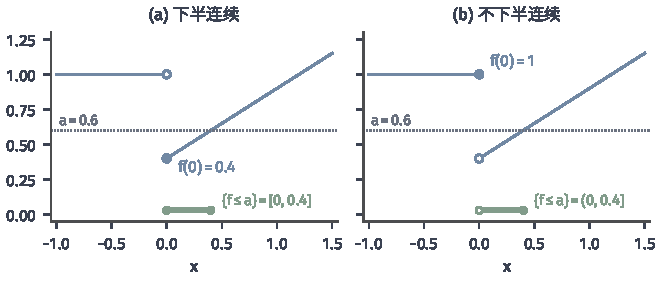
\includegraphics[width=112mm]{figures/03-optimization-evolution-and-signals/01-optimization/matplotlib/c1-lsc-gap/figure.pdf}
  \caption{下半连续与下水平集的缺口。两个函数在$x<0$时都等于$1$，在$x>0$时都等于$0.4+0.5x$，只在$x=0$处取值不同（实心点）。灰色点线是水平$a=0.6$，绿色线段是下水平集$\{f\leq0.6\}$。(a) $f(0)=0.4$，函数下半连续，下水平集为闭区间$[0,0.4]$；(b) $f(0)=1$，在$0$处向上跳，不下半连续，下水平集$(0,0.4]$缺少端点。}
  \label{fig:opt-prob-lsc-gap}
\end{figure}

\paragraph{紧可行域上的存在定理}
三个环节齐备，就得到存在性。

\begin{theorem}[紧可行域上的最小值]
\label{thm:opt-prob-compact-existence}
设$C\subseteq\mathbb R^d$非空且紧，$f:C\to\mathbb R\cup\{+\infty\}$在$C$上下半连续，且至少有一点$\bm x\in C$使$f(\bm x)<+\infty$。则$f^\star=\inf_{\bm x\in C}f(\bm x)$是有限实数，且最优解集合非空。
\end{theorem}

\begin{proof}
由假设$f^\star<+\infty$。取最小化序列$\bm x^{(k)}\in C$：$f^\star$有限时要求$f(\bm x^{(k)})\leq f^\star+1/k$，$f^\star=-\infty$时要求$f(\bm x^{(k)})\leq-k$。$C$紧，故有子列$\bm x^{(k_j)}\to\bm x^\star\in C$。由下半连续，
\[
  f(\bm x^\star)\leq\liminf_{j\to\infty}f(\bm x^{(k_j)})=f^\star.
\]
若$f^\star=-\infty$，上式给出$f(\bm x^\star)=-\infty$，与$f$不取$-\infty$矛盾，所以$f^\star$有限。又$\bm x^\star$可行，$f(\bm x^\star)\geq f^\star$；两个不等式合起来得$f(\bm x^\star)=f^\star$，$\bm x^\star$是最优解。
\end{proof}

资源分配的可行域是四条闭半平面的交，有界且闭，目标是线性函数，因而连续；定理~\ref{thm:opt-prob-compact-existence}立即保证最优解存在。这个结论不需要知道最优解在$(2,2)$，它只确认值得去找。

\paragraph{三个环节各自的失效}
图~\ref{fig:opt-prob-existence-failures}用三个例子分别拆掉一个环节。(a) 在$C=(0,1]$上最小化$f(x)=x$：最小化序列$2^{-k}$收敛到$0$，但$0$不在$C$中，失败在“极限可行”；$C$有界但不闭。(b) 在$C=[1,\infty)$上最小化$f(x)=1/x$：$C$闭但无界，序列$2^k$的目标值趋于下确界$0$，自身却逃向无穷远，没有收敛子列，失败在“序列留在有界区域”。(c) 在紧集$C=[-1,1]$上，令$f(x)=x^2$（$x\neq0$）、$f(0)=0.6$：序列$1/k$收敛到$0$，目标值趋于$0$，但极限处函数值跳到$0.6$，下确界$0$未被达到，失败在“比较传到极限”，因为$f$在$0$处不下半连续。三个条件缺一不可，但它们都只是充分条件：例如$f(x)=x^2$在无界的$\mathbb R$上仍有最小点。

\begin{figure*}[!htbp]
  \centering
  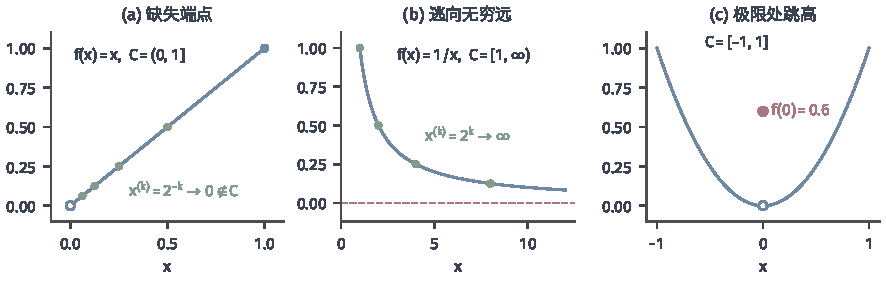
\includegraphics[width=150mm]{figures/03-optimization-evolution-and-signals/01-optimization/matplotlib/c1-existence-failures/figure.pdf}
  \caption{存在性论证的三个环节分别失效。绿点是最小化序列。(a) $f(x)=x$，$C=(0,1]$：序列$2^{-k}$趋于不可行的端点$0$（空心点）。(b) $f(x)=1/x$，$C=[1,\infty)$：序列$2^k$逃向无穷远，目标值趋于红色虚线$0$。(c) $f(x)=x^2$（$x\neq0$），$f(0)=0.6$，$C=[-1,1]$：序列趋于$0$时目标值趋于$0$，但$f(0)$跳高到$0.6$（红点），空心点处的值$0$无人取得。}
  \label{fig:opt-prob-existence-failures}
\end{figure*}

\subsection{强制性与紧下水平集}
\label{sec:opt-prob-coercive}

\paragraph{无界可行域怎么办}
最小二乘的可行域是整个$\mathbb R^d$，它不紧，定理~\ref{thm:opt-prob-compact-existence}不能直接用。但我们并不需要整个可行域紧，只需要最小化序列被关在某个紧集里。取一个可行点$\bar{\bm x}$，凡是目标值比$f(\bar{\bm x})$还高的点都不可能是最优解，可以直接丢掉；剩下的是下水平集$\{\bm x\in C:f(\bm x)\leq f(\bar{\bm x})\}$。如果这个集合紧，问题就回到紧集上。它闭的条件已由引理~\ref{lem:opt-prob-lsc-sublevel}给出，还缺有界：目标必须在远处足够高，使“不太差的点”不会跑到无穷远。

\begin{definition}[强制性]
\label{def:opt-prob-coercive}
设$C\subseteq\mathbb R^d$，$f:C\to\mathbb R\cup\{+\infty\}$。若对$C$中任意满足$\lVert\bm x^{(k)}\rVert_2\to\infty$的序列都有$f(\bm x^{(k)})\to+\infty$，就称$f$在$C$上是\term{强制的}（coercive）。$C$有界时，这个条件自动成立。
\end{definition}

强制性等价于：每个下水平集都有界。若某个水平$a$的下水平集无界，从中取范数趋于无穷的序列，其目标值始终不超过$a$，与强制性矛盾；反过来，若各下水平集都有界，而$\lVert\bm x^{(k)}\rVert_2\to\infty$，则对任意$a$，序列最终离开水平$a$的下水平集，即最终$f(\bm x^{(k)})>a$，所以$f(\bm x^{(k)})\to+\infty$。

\begin{theorem}[强制目标的最小值]
\label{thm:opt-prob-coercive-existence}
设$C\subseteq\mathbb R^d$非空且闭，$f:C\to\mathbb R\cup\{+\infty\}$在$C$上下半连续且强制，并且存在$\bar{\bm x}\in C$使$f(\bar{\bm x})<+\infty$。则$f^\star$是有限实数，且最优解集合非空。
\end{theorem}

\begin{proof}
令$K=\{\bm x\in C:f(\bm x)\leq f(\bar{\bm x})\}$。它含有$\bar{\bm x}$，非空；由引理~\ref{lem:opt-prob-lsc-sublevel}，它是闭集；由强制性，它有界。于是$K$紧，$f$限制在$K$上仍下半连续，定理~\ref{thm:opt-prob-compact-existence}给出$\bm x^\star\in K$，使$f(\bm x^\star)=\min_Kf\leq f(\bar{\bm x})$。对$C\setminus K$中的点，$f(\bm x)>f(\bar{\bm x})\geq f(\bm x^\star)$。所以$\bm x^\star$是$f$在整个$C$上的最小点，$f^\star=f(\bm x^\star)$有限。
\end{proof}

证明中各条件的分工很清楚：强制性让下水平集有界，留住了序列；$C$闭与下半连续让下水平集闭，留住了极限；剩下的工作交给紧集上的定理。

\paragraph{回到最小二乘}
对式~\eqref{eq:opt-prob-ridge}逐项核对。$f$是多项式，处处有限，因而适当且连续；$C=\mathbb R^d$闭，加上非负约束后$C=\{\bm x:\bm x\geq\bm 0\}$也是闭集。当$\lambda>0$时，$f(\bm x)\geq\frac{\lambda}{2}\lVert\bm x\rVert_2^2$，范数趋于无穷时目标趋于无穷，$f$强制。由定理~\ref{thm:opt-prob-coercive-existence}，无论是否加非负约束，最优解都存在。

$\lambda=0$时情况不同。在最小二乘实例中，$f(\bm x)=\frac12(x_1+x_2-2)^2$沿方向$(1,-1)$保持不变：取$\bm x^{(k)}=(1+k,1-k)$，范数趋于无穷而$f=0$，所以$f$不强制，水平$1$的下水平集是一条无界的带。图~\ref{fig:opt-prob-ls-sublevel}比较了两种情形：$\lambda=0.5$时同一水平的下水平集收缩为一个椭圆，$\lambda=0$时则沿最优解直线无限延伸。然而$\lambda=0$时最优解仍然存在——整条直线$x_1+x_2=2$都是。这说明强制性只是充分条件；对一般的$\bm A$，无正则最小二乘总有解，这由正规方程的可解性保证，而不是由强制性保证（可参考\BookChapterRef{chap:linear-equations-and-optimization}{卷一“线性方程与矩阵方程”章}）。若$\bm A$列满秩，则对$\bm x\neq\bm 0$有$\bm A\bm x\neq\bm 0$，在单位球面上取最小值可得常数$\sigma>0$使$\lVert\bm A\bm x\rVert_2\geq\sigma\lVert\bm x\rVert_2$，此时即使$\lambda=0$，$f$也强制。

\begin{figure*}[!htbp]
  \centering
  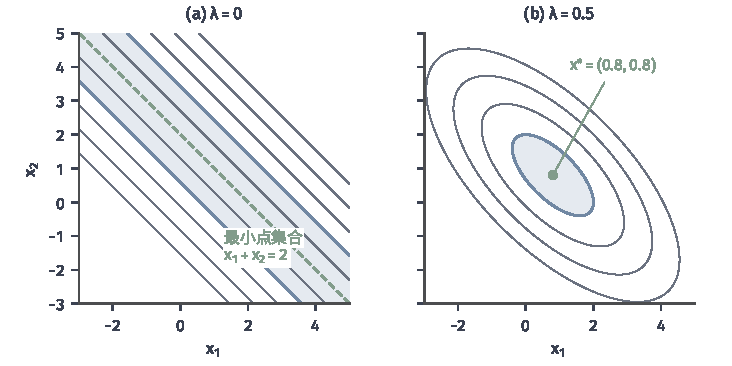
\includegraphics[width=124mm]{figures/03-optimization-evolution-and-signals/01-optimization/matplotlib/c1-ls-sublevel/figure.pdf}
  \caption{最小二乘实例$f(\bm x)=\frac12(x_1+x_2-2)^2+\frac{\lambda}{2}\lVert\bm x\rVert_2^2$的下水平集。浅蓝区域及其蓝色边界是$\{f\leq1\}$，灰线是$f=0.25,2.25,4,6.25$的等值线。(a) $\lambda=0$：下水平集是两条平行线之间的无界带，最优解集合是绿色虚线$x_1+x_2=2$。(b) $\lambda=0.5$：下水平集是有界椭圆，唯一最优解为$\bm x^\star=(0.8,0.8)$，最优值为$0.4$。}
  \label{fig:opt-prob-ls-sublevel}
\end{figure*}

\paragraph{有限维的边界}
整个论证依赖“有界闭集紧”这一有限维性质。在无限维空间中它不成立：例如平方可和序列空间中，第$k$个坐标为$1$、其余为$0$的单位向量$\bm e_k$两两距离都是$\sqrt2$，它们都在闭单位球中，却没有收敛子列。于是即使目标强制、下水平集有界闭，最小化序列也可能没有极限。处理函数空间中的存在性需要更弱的收敛概念，这是第~\ref{chap:opt-functional}章的任务。
